\section{误差来自何处}

简单的模型有着较大的偏差(bias),使用相同模型,不同数据得到的最优函数$f^*$的取值区间可能不包括理论最优解$\hat{f}$,因此偏差较大。而对于过于复杂的模型,又容易产生对数据的过拟合,出现大的方差。
对于复杂模型,多次实验求取的模型均值能够更加接近理论解$\hat{f}$,但同时一个模型对于新的测试集数据容易产生大的误差,此时误差主要来自方差(variance)。偏差与误差的形象解释如图\ref{fig:bias_and_variance}所示:

\begin{figure}
	\centering

	{\subcaptionbox{误差之偏差}{%
	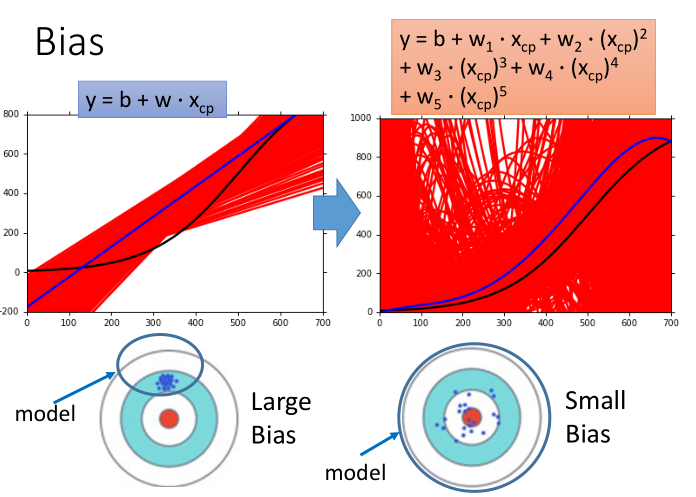
\includegraphics[scale=0.4]{pic/bias.png}}\qquad
	\subcaptionbox{误差之方差}{%
	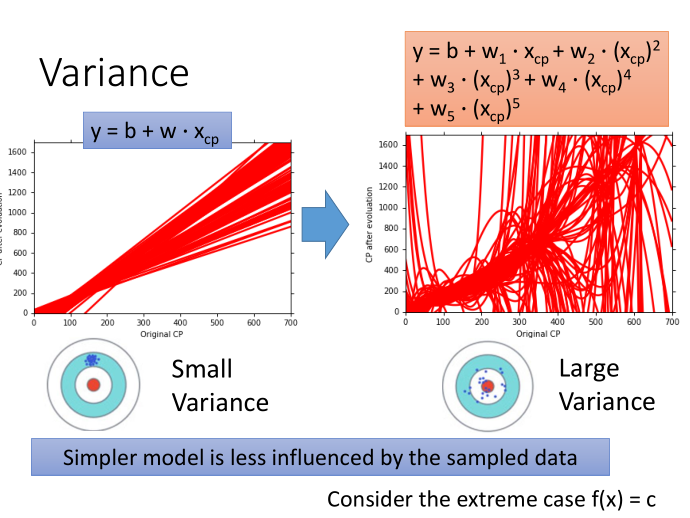
\includegraphics[scale=0.4]{pic/variance.png}}
	}
	\caption{bias VS variance}
	\label{fig:bias_and_variance}
\end{figure}


